\documentclass{beamer}
\let\vec\mathbf
\mode<presentation>
\usepackage{amsmath}
\usepackage{amssymb}
%\usepackage{advdate}
\usepackage{adjustbox}
%\usepackage{subcaption}
\usepackage{xparse}
\usepackage{enumitem}
\usepackage{multicol}
\usepackage{mathtools}
\usepackage{listings}
\usepackage{url}
\usepackage{gvv}
\usetheme{Boadilla}
\usecolortheme{lily}
\setbeamertemplate{footline}
{
  \leavevmode%
  \hbox{%
  \begin{beamercolorbox}[wd=\paperwidth,ht=2.25ex,dp=1ex,right]{author in head/foot}%
    \insertframenumber{} / \inserttotalframenumber\hspace*{2ex} 
  \end{beamercolorbox}}%
  \vskip0pt%
}
\setbeamertemplate{navigation symbols}{}
\providecommand{\nCr}[2]{\,^{#1}C_{#2}} % nCr
\providecommand{\nPr}[2]{\,^{#1}P_{#2}} % nPr
\providecommand{\mbf}{\mathbf}
\providecommand{\pr}[1]{\ensuremath{\Pr\left(#1\right)}}
\providecommand{\qfunc}[1]{\ensuremath{Q\left(#1\right)}}
\providecommand{\sbrak}[1]{\ensuremath{{}\left[#1\right]}}
\providecommand{\lsbrak}[1]{\ensuremath{{}\left[#1\right.}}
\providecommand{\rsbrak}[1]{\ensuremath{{}\left.#1\right]}}
\providecommand{\brak}[1]{\ensuremath{\left(#1\right)}}
\providecommand{\lbrak}[1]{\ensuremath{\left(#1\right.}}
\providecommand{\rbrak}[1]{\ensuremath{\left.#1\right)}}
\providecommand{\cbrak}[1]{\ensuremath{\left\{#1\right\}}}
\providecommand{\lcbrak}[1]{\ensuremath{\left\{#1\right.}}
\providecommand{\rcbrak}[1]{\ensuremath{\left.#1\right\}}}
\theoremstyle{remark}

\providecommand{\res}[1]{\Res\displaylimits_{#1}} 
\providecommand{\norm}[1]{\lVert#1\rVert}
\providecommand{\mtx}[1]{\mathbf{#1}}

\providecommand{\fourier}{\overset{\mathcal{F}}{ \rightleftharpoons}}
%\providecommand{\hilbert}{\overset{\mathcal{H}}{ \rightleftharpoons}}
\providecommand{\system}{\overset{\mathcal{H}}{ \longleftrightarrow}}
	%\newcommand{\solution}[2]{\textbf{Solution:}{#1}}
%\newcommand{\solution}{\noindent \textbf{Solution: }}
\providecommand{\dec}[2]{\ensuremath{\overset{#1}{\underset{#2}{\gtrless}}}}

\title{Matrices in Geometry - 5.8.33}
\author{EE25BTECH11035  Kushal B N}
\date{Oct, 2025}

\begin{document}

\maketitle

\section{Problem Statement}
\begin{frame}
\frametitle{Problem Statement}
Draw the graphs of the equations $5x - y = 5$ and $3x - y = 3$.\\ Determine the co-ordinates of the vertices of the triangle formed by these lines and the y-axis.
\end{frame}

\section{Solution}
\begin{frame}{Solution}
Given,\\
The lines $\myvec{5&-1}\myvec{x\\y} = 5$ and $\myvec{3&-1}\myvec{x\\y} = 3$.
The y-axis $\myvec{1&0}\myvec{x\\y} = 0$.

Solving for the intersection of the two lines
\begin{equation}
    \myvec{5&-1\\3&-1}\myvec{x\\y} = \myvec{5\\3}
\end{equation}
Forming the augmented matrix for solving this,
\begin{equation}
    \augvec{2}{2}{5&-1&5\\3&-1&3}
\end{equation}

\begin{equation}
    \xleftrightarrow{R_1 \leftarrow R_1 - R_2} \augvec{2}{2}{2&0&2\\3&-1&3} \xleftrightarrow{R_2 \leftarrow -R_2} \augvec{2}{2}{2&0&2\\-3&1&-3}
\end{equation}
\end{frame}

\begin{frame}{Solution}
\begin{equation}
    \xleftrightarrow{R_1 \leftarrow \frac{R_1}{2}} \augvec{2}{2}{1&0&1\\-3&1&-3} \xleftrightarrow{R_2 \leftarrow R_2 + 3R_1} \augvec{2}{2}{1&0&1\\0&1&0}
\end{equation}

\begin{equation}
    \implies \myvec{x\\y} = \myvec{1\\0}
\end{equation}

Now, the intersection of the two lines with the y-axis,

First line:
\begin{equation}
    \myvec{5&-1\\1&0}\myvec{x\\y} = \myvec{5\\0}
\end{equation}

Forming augmented matrix and solving,

\begin{equation}
  \augvec{2}{2}{5&-1&5\\1&0&0} \xleftrightarrow{R_1 \leftarrow R_2} \augvec{2}{2}{1&0&0\\5&-1&5}
\end{equation}
\end{frame}

\begin{frame}{Solution}
\begin{equation}
    \xleftrightarrow{R_2 \leftarrow R_2 - 5R_1} \augvec{2}{2}{1&0&0\\0&-1&5} \xleftrightarrow{R_2 \leftarrow -R_2} \augvec{2}{2}{1&0&0\\0&1&-5}
\end{equation}

\begin{equation}
    \implies \myvec{x\\y} = \myvec{0\\-5}
\end{equation}
Second Line:
\begin{equation}
    \myvec{1&0\\3&-1}\myvec{x\\y} = \myvec{0\\3}
\end{equation}
Forming the augmented Matrix,
\begin{equation}
    \augvec{2}{2}{1&0&0\\3&-1&3} \xleftrightarrow{R_2 \leftarrow R_2 - 3R_1} \augvec{2}{2}{1&0&0\\0&-1&3}
\end{equation}

\begin{equation}
    \xleftrightarrow{R_2 \leftarrow -R_2} \augvec{2}{2}{1&0&0\\0&1&-3}
\end{equation}

\begin{equation}
    \implies \myvec{x\\y} = \myvec{0\\-3}
\end{equation}
\end{frame}

\section{Conclusion}
\begin{frame}{Conclusion}
$\therefore$ The coordinates of the vertices of the triangle formed by these lines anad the y-axis are $\myvec{1\\0}$, $\myvec{0\\-5}$ and $\myvec{0\\-3}$.

The graph of the system of equations:\\

\begin{figure}[H]
    \centering
    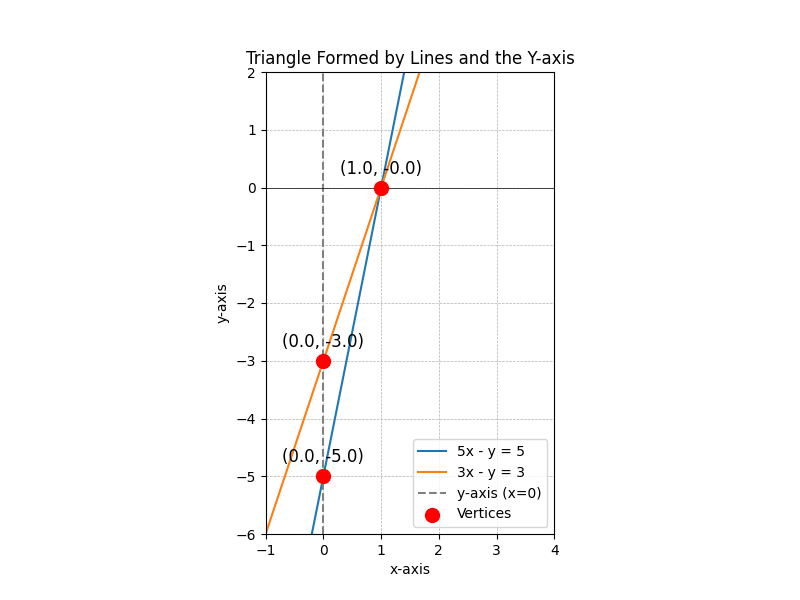
\includegraphics[width=0.60\columnwidth]{figs/1.png}
    \caption{Figure for 5.8.33}
\end{figure}
\end{frame}
\end{document}
